\documentclass[tikz,border=2pt]{standalone}
\usepackage[T1]{fontenc}
\usepackage{tgheros}
\usepackage{inconsolata}
\renewcommand{\familydefault}{\sfdefault}
\usetikzlibrary{arrows.meta,fit,positioning,shapes.symbols}
\pgfdeclarelayer{region}
\pgfdeclarelayer{cloud}
\pgfsetlayers{region,cloud,main}

\definecolor{diskgreen}{HTML}{B6D7A8}
\definecolor{cloudblue}{HTML}{CFE2F3}
\definecolor{formatyellow}{HTML}{FFE599}
\definecolor{functionblue}{HTML}{6FA8DC}
\definecolor{memoryred}{HTML}{EA9999}

\begin{document}
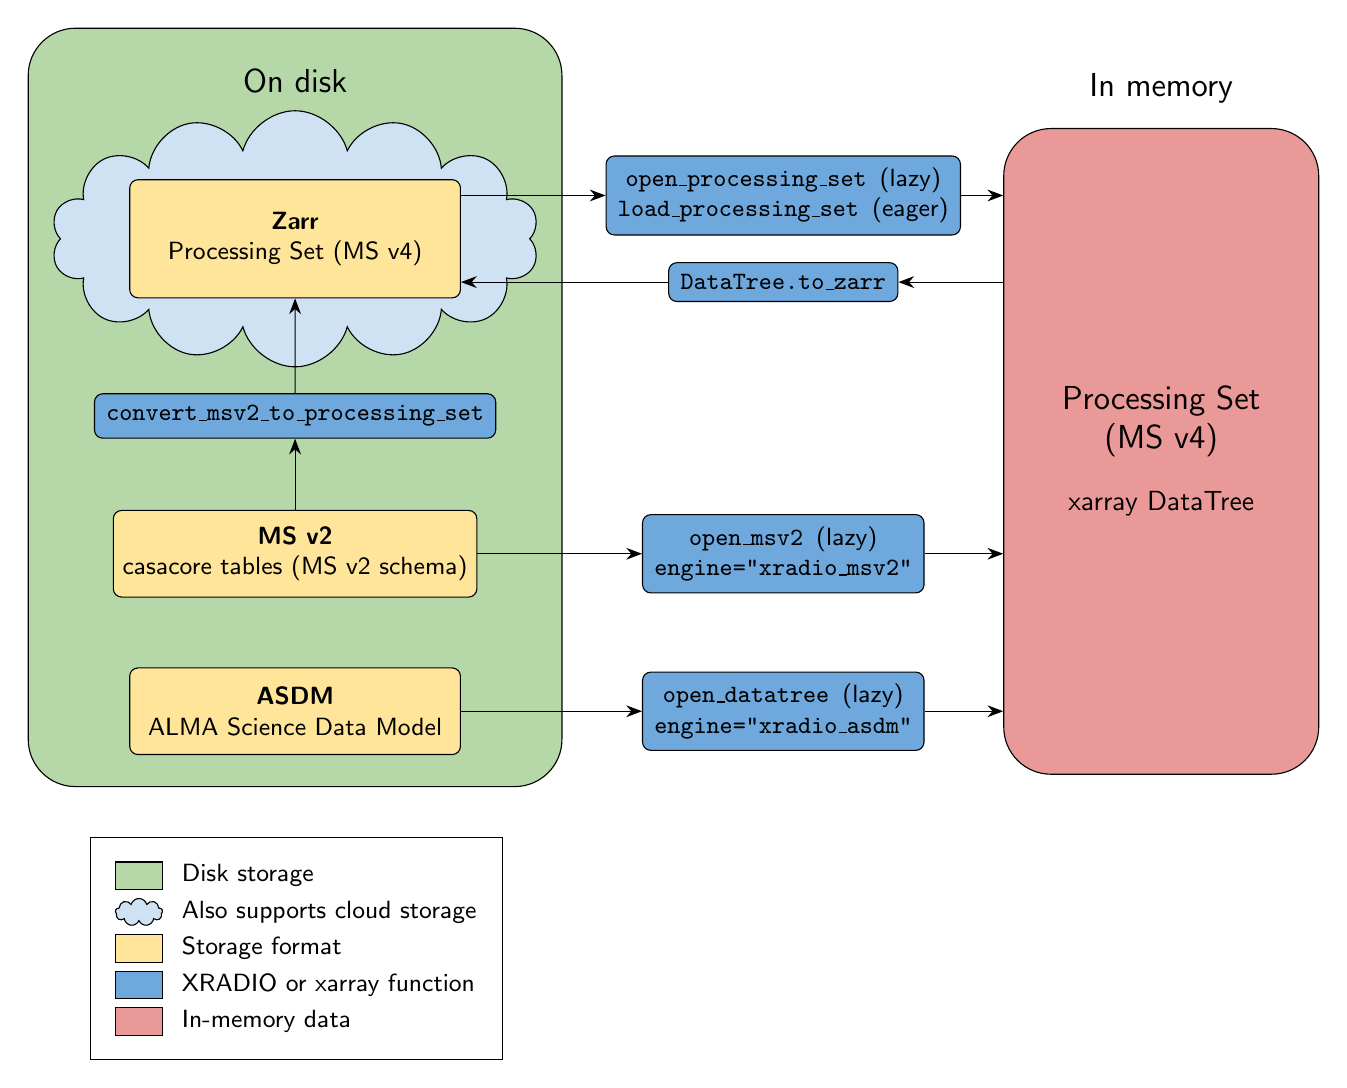
\begin{tikzpicture}[
    font=\small,
    format/.style={draw, fill=formatyellow, rounded corners=3pt,
      minimum width=4.2cm, minimum height=1.1cm, align=center},
    function/.style={draw, fill=functionblue, rounded corners=3pt,
      inner sep=1.5mm, align=center, font=\ttfamily\small},
    to/.style={-{Stealth[length=2mm]}},
    region/.style={draw, rounded corners=6mm, inner sep=4mm},
    title/.style={font=\large},
  ]
  \node[format, minimum height=1.5cm] (zarr) at (0, 5)
    {\textbf{Zarr}\\ Processing Set (MS v4)};
  \node[format] (msv2) at (0, 1)
    {\textbf{MS v2}\\ casacore tables (MS v2 schema)};
  \node[format] (asdm) at (0, -1)
    {\textbf{ASDM}\\ ALMA Science Data Model};
  \begin{pgfonlayer}{cloud}
    \node[cloud, cloud puffs=14, aspect=2.6, draw, fill=cloudblue,
      fit=(zarr), inner sep=0pt] (cloud) {};
  \end{pgfonlayer}
  \node[function] (convert) at (0, 2.75) {convert\_msv2\_to\_processing\_set};
  \draw[to] (msv2) -- (convert);
  \draw[to] (convert) -- (cloud.south |- zarr.south);

  \node[draw, fill=memoryred, rounded corners=6mm, minimum width=4cm,
    minimum height=8.2cm, align=center, font=\large] (ps) at (11, 2.3)
    {Processing Set\\ (MS v4)\\[3mm] \normalsize xarray DataTree};

  \node[function] (open ps) at (6.2, 5.55)
    {open\_processing\_set \textsf{(lazy)}\\ load\_processing\_set \textsf{(eager)}};
  \node[function] (to zarr) at (6.2, 4.45) {DataTree.to\_zarr};
  \node[function] (open msv2) at (6.2, 1)
    {open\_msv2 \textsf{(lazy)}\\ engine="xradio\_msv2"};
  \node[function] (open asdm) at (6.2, -1)
    {open\_datatree \textsf{(lazy)}\\ engine="xradio\_asdm"};
  \draw[to] (zarr.east |- open ps) -- (open ps);
  \draw[to] (open ps) -- (ps.west |- open ps);
  \draw[to] (ps.west |- to zarr) -- (to zarr);
  \draw[to] (to zarr) -- (zarr.east |- to zarr);
  \draw[to] (msv2) -- (open msv2);
  \draw[to] (open msv2) -- (ps.west |- open msv2);
  \draw[to] (asdm) -- (open asdm);
  \draw[to] (open asdm) -- (ps.west |- open asdm);

  \node[title, above=1mm of cloud] (disk title) {On disk};
  \node[title, above=2mm of ps] {In memory};
  \begin{pgfonlayer}{region}
    \node[region, fill=diskgreen, fit=(disk title) (cloud) (asdm)] {};
  \end{pgfonlayer}

  \matrix[draw, anchor=north west, column sep=2mm, row sep=1mm, inner sep=3mm,
      nodes={anchor=west, inner sep=1pt}] at (-2.6, -2.6) {
    \node[draw, fill=diskgreen, minimum width=6mm, minimum height=3.5mm] {}; &
      \node {Disk storage}; \\
    \node[cloud, cloud puffs=9, aspect=1.8, draw, fill=cloudblue,
      minimum width=6mm, minimum height=3.5mm] {}; &
      \node {Also supports cloud storage}; \\
    \node[draw, fill=formatyellow, minimum width=6mm, minimum height=3.5mm] {}; &
      \node {Storage format}; \\
    \node[draw, fill=functionblue, minimum width=6mm, minimum height=3.5mm] {}; &
      \node {XRADIO or xarray function}; \\
    \node[draw, fill=memoryred, minimum width=6mm, minimum height=3.5mm] {}; &
      \node {In-memory data}; \\
  };
\end{tikzpicture}
\end{document}
